\documentclass[10pt]{article}

\usepackage{graphicx}
\usepackage{amsmath}
\usepackage{verbatim}
\usepackage{mathrsfs}
\usepackage{url}
\usepackage{natbib}
\usepackage{subfig}

\let\proglang=\textsf
\newcommand{\pkg}[1]{{\fontseries{b}\selectfont #1}}

\newcommand{\E}{\mathsf{E}}
\newcommand{\VAR}{\mathsf{VAR}}
\newcommand{\COV}{\mathsf{COV}}
\newcommand{\SD}{\mathsf{SD}}
\newcommand{\Prob}{\mathsf{P}}
\newcommand{\code}[1]{\texttt{#1}}

\author{Vincent Dorie\\Columbia University \And
        Andrew Gelman\\Columbia University}
\title{\pkg{blmer}: Weakly Informative Covariance Priors for
  Multilevel Linear Models in \proglang{R}}

\begin{document}

\begin{abstract}
The \pkg{blmer} package for \proglang{R} computes maximum a posteriori estimates for
  the covariance parameters in multilevel linear models, using weakly informative priors
  that guarantee a positive definite result. Additionally, fully
  Bayesian inference is possible through the specification of
  priors over additional parameters, a posterior sampler, and cross validation. It builds off of, and is
  cross-compatible with the popular multilevel/mixed effects
  regression \proglang{R} package \pkg{lme4}. \pkg{blmer} supports a
  variety of prior distributions and covariance decompositions, and
  incorporates an expressive syntax that is designed to be familiar
  to users of regression functions in \proglang{R}.
\end{abstract}

\section{Introduction}

In multilevel models, maximum likelihood estimates of the covariance
matrices for the modeled coefficients (also known as ``random
effects'') can be at the boundary of the parameter
space. Estimation in this case is problematic as the likelihood
surface can be flat, slowing optimization and providing innaccurate
estimates of standard errors. For a discussion of the the problems
associated with degenerate covariance estimates in multilevel
models, see (TODO: reference our other paper?).

As a solution, the \pkg{blmer} package for \proglang{R} \citep{r_team:2010:R} imposes
prior distributions over the relevant covariance matrices such that there is
zero probability mass associated with the boundary. Excepting this
behavior, the prior distributions have been chosen to be otherwise
vague and come with default settings that should be suitable in most applications. With these priors,
\pkg{blmer} is able to gently shift estimates that are at the boundary
away from $0$ while leaving other parameters roughly
unaffected. Furthermore, \pkg{blmer} permits the user to specify
prior distributions over the remaining model parameters, obtain samples from
the posterior, and estimate the prediction error for new
samples using cross validation. Combined, these tools provide a fully Bayesian approach to
multilevel linear models.

As there already exists for \proglang{R} a popular and efficient means
of fitting multilevel models using maximum likelihood, one of our key computational goals was to be
cross-compatible with, and to build off of the \pkg{lme4} package
\citep{bates:2010:lme4}. Users of \pkg{lme4} will find in \pkg{blmer} a
near-identical user interface and results contained in S4 objects that
inherit from that package's \code{mer} object model.

Finally, we have attempted to create a prior specification language
that mirrors the simplicity and expressiveness of \proglang{R}'s
model description syntax to setup the prior's structure, while combining the usefulness of
named lists to set hyperparameters.

\section[Multilevel linear models]{Multilevel linear models}

While multilevel models have been well explicated elsewhere
(TODO: references), we will briefly go over the model specification so that
we can mathematically highlight how \pkg{blmer} differs from its predecessors. While
what follows is for a linear model, generalized linear models are
essentially similar in parameterization, except that they may lack an
observation-level variance component.

Multilevel models apply to situations in which observational units can
be naturally grouped together. There may be different grouping
``factors'' that apply. For
example, a poll respondant might be grouped with other individuals by his or her race and/or
state. Suppose that there are $K$ such grouping factors,
and that the number of potential groups at level $k$ is denoted as
$J_k$. Each observational unit then has $K$ memberships, and we choose to
denote which one of the $J_k$ groups the $i$th
observation belongs at the $k$th level by writing: $[i]_k$.

Now assume that we have $y_i, i=1, \ldots, N$ observations and each is associated
with a vector of predictors, $x_i^\top$. Furthermore, for each of the
$k=1,\ldots,K$ factors and for each of the $j=1, \ldots, J_k$ groups
in that factor, we have another vector of predictors, $z_{jk}^\top$. A
multilevel linear model would then be given by:

\begin{align*}
y_i \mid \theta & \overset{\text{ind}}{\sim} N\left(x_i^\top\beta +
  \sum_{k=1}^Kz_{[i]_kk}^\top\theta_{[i]_kk}, \sigma^2 \right), i=1,
\ldots, N, \\
\theta_{jk} \mid \Sigma_k & \overset{\text{iid}}{\sim} N\left(0, \Sigma_k\right),
j=1, \ldots, J_k, k=1, \ldots, K.
\end{align*}

\noindent Our principle concern is with imposing priors $p(\Sigma_k)$ such that
$\lim_{|\Sigma_k| \rightarrow 0} p(\Sigma_k) = 0$. We also otherwise
generalize the above by imposing priors $p(\beta)$ and $p(\sigma^2)$.

As \pkg{lme4} maximizes the likelihood using numerical optimization
on the covariance matrices of the latent variables, obtaining a
posterior mode requires nothing more than ``penalizing'' that
likelihood calculation by the contribution of the prior.

Priors and $\beta$ and $\sigma^2$ have also been
implemented. Conjugate families for these parameters are incorporated
as pseudo-data, while non-conjugate families require expanding the
parameter space used in optimization.

\subsection[Covariance decompositions]{Covariance decompositions}

In addition to imposing a prior directly on the covariance matrices of
the model, we have also implemented two covariance decompositions
which give the use more fine-grained control. The ``correlation''
decomposition attempts to treat the covariance matrix as a set of standard
deviations and correlations, while the ``spectral'' decomposition
breaks the matrix into its eigenvectors and eigenvalues.

The correlation decomposition is given by: $\Sigma = SRS$, for $S$
a diagonal matrix of strictly positive elements and $R$ a correlation
matrix. As optimizing over a correlation matrix is a highly
constrained problem, we instead let $R$ be any positive definite
matrix. Consequently, the correlation decomposition corresponds to a
redundant, multiplicative parameterization. (TODO: redundant, multiplicative
parameterization are good + citation).

Alternatively, the spectral decomposition can be written as $\Sigma =
Q\Lambda Q^\top$, where $Q$ is an orthogonal matrix comprising the
eigenvectors of $\Sigma$, and $\Lambda$ is a
diagonal matrix of eigenvalues. 

Chosing one of the above decompositions alters the posterior mode
returned by \pkg{blmer} to that of the decomposition itself. In the
first case, this is necessary as the imposed prior involves an
integral which may or may not be tractible. In the second, imposing
priors on eigenvalues independently induces a prior on the original
scale that has infinite mass in the limit as eigenvalues approach each
other, which in turn complicates optimization. (TODO: reference as to
why this is OK/good?)

\section[Fitting models]{Fitting models}

\pkg{blmer} was designed to familiar to users of \pkg{lme4}. A \code{blmer} S4 object extends the \code{mer} class, and
consequently inherits all of the same functionality. Fitting a model
in \pkg{blmer} is achieved by modifying a call to the \code{lmer()} or \code{glmer()} function
with the addition of several new arguments.

\subsection[Calling blmer]{Calling \code{blmer()}}

The prototype for the \code{blmer()} and \code{bglmer()} functions are given below:

\begin{verbatim}
blmer(formula, data, family = NULL, REML = TRUE, control = list(),
      start = NULL, verbose = FALSE, doFit = TRUE, subset, weights,
      na.action, offset, contrasts = NULL, model = TRUE, x = TRUE,
      cov.prior = NULL, fixef.prior = NULL, var.prior = NULL)
bglmer(formula, data, family = gaussian, start = NULL, verbose = FALSE,
       nAGQ = 1, doFit = TRUE, subset, weights, na.action, offset,
       contrasts = NULL, model = TRUE, control = list(),
       cov.prior = NULL, fixef.prior = NULL)
\end{verbatim}

\noindent Note that except for the last lines, these are identical to
the prototypes for \code{lmer()} and \code{glmer()}, as of version
0.999375-37 of the \pkg{lme4} package.

The formats for the new arguments are all character strings (TODO:
figure out if character strings are necessary) of a
syntax that will be described below, but as an
overview, the new arguments are:

\begin{itemize}
\item \code{cov.prior}: a prior on the covariance matrices of the
  modeled coefficients. The covariance matrices are denoted as
  $\Sigma$ in the above formulation. Applies to both \code{blmer()} and \code{bglmer()}.
\item \code{fixef.prior}: a prior on the unmodeled regression
  coefficients, or fixed effects ($\beta$). Also applies to both functions, but
  cannot be used in a call to \code{blmer()} if the \code{REML}
  argument is \code{TRUE}.
\item \code{var.prior}: prior on the observation level variance
  component, $\sigma^2$. Only applies to calls to \code{blmer()} as
  generalized linear models do not have this parameter (TODO: overdispersion?).
\end{itemize}

As priors require parameters of their own, we have adopted the
named-element list format used by \proglang{R}, mimicking the syntax for function
calls.

\subsection[Covariance prior]{Covariance prior}

\begin{table}
\begin{center}{\scriptsize
\begin{tabular}{llllll}
type & restriction & posterior & families & options \& \\ 
& & mode & & defaults \\ \hline
\vspace{.05in} none & none & $\Sigma$ & $p(\Sigma) \propto 1$ & none \\
direct & $\dim{\Sigma}=1$ & $\Sigma_{[11]}$ or &
\code{gamma}, & \code{shape = 2}, \\
& & $\sqrt{\Sigma_{[11]}}$ & & \code{rate = 1 / sd(y)}, \\
& & & & \code{posterior.scale = }\verb/'sd'/ \\
& & &\code{inverse.gamma} & \code{shape = 1 / 2}, \\
& & & & \code{scale = 3 * sd(y) / 2}, \\ 
& & & & \code{posterior.scale = }\verb/'sd'/ \\
direct & $\dim{\Sigma} > 1$ & $\Sigma$ & \code{wishart}, & \code{df =
  dim(sigma) + 3}, \\
& & & & \code{scale = diag(sd(y) / 2, dim(sigma))} \\
& & & \code{inverse.wishart} & \code{df = dim(sigma) - 1 / 2}, \\ 
& & & & \code{inverse.scale =
diag(3 * sd(y), dim(sigma))} \\

\code{correlation} & none & $S$, $R$ or            & $S_{[jj]} \sim $ \code{gamma}, & same as \code{gamma} above \\
                             &          & $S^{1/2}, R$            & $S_{[jj]} \sim $\code{inverse.gamma} & same as \code{inverse.gamma} above \\
                             &          & where  & $R \sim $ \code{wishart} & same as \code{wishart} above \\
                             &          & $\Sigma = SRS$,       &  $R \sim $ \code{inverse.wishart} & same as \code{inverse.wishart} above \\ 
                             &          & $S$ diagonal, & & default
                             families: $S_{[jj]} \overset{iid}{\sim} $
                             \code{gamma}, $R \sim $ \code{wishart}   \\ 
                             &          & $R$ pos. def.\\
\code{spectral}     & none & $Q, \Lambda$ or   & $\Lambda_{[jj]} \sim $ \code{gamma} & same as above, but \code{posterior.scale  = }\verb/'var'/ \\
                             &          & $Q, \Lambda^{1/2}$ & $\Lambda_{[jj]} \sim $ \code{inverse.gamma} & same as above, but \code{posterior.scale = }\verb/'var'/ \\
                             &          & where & $p(Q) \propto 1$ & none\\
                            &           & $\Sigma = Q\Lambda Q^\top$,
                            & & default
                             families: $\Lambda_{[jj]} \overset{iid}{\sim} $
                             \code{gamma} \\
                            &           & $Q$ orthogonal, \\
                            &           & $\Lambda$ diagonal
\end{tabular}
}
\end{center}
\caption{Types, families, and options for priors on covariance
  components corresponding to the unobserved variables. The defaults
  correspond to fitting a standard, multilevel linear model. In the
  case of a generalized linear model, any reference to the standard
  deviation of the observations is replaced by 1. (TODO: seems
  reasonable for logistic. What about other glms?)}
\label{tab:covariance_prior_options}
\end{table}

The principal difficulty in specifying a prior on $\Sigma$ is that there
are separately estimated covariance matrices for each of the $K$
grouping factors. To afford the user more flexibility, priors can be specified as a default
that will apply to all grouping factors or applied directly by the
level name. To specify a prior that applies to a specific, named
grouping factor, one passes to \code{blmer()} a character string of
the format:

\begin{verbatim}
factor.name ~ prior.type(options.list)
\end{verbatim}

\noindent Conversely, to specify a default prior that should apply to
all grouping factors, the correct format is simply:
\code{prior.type(options.list)}.

The different prior types, options, and defaults are enumerated in Table~\ref{tab:covariance_prior_options}. Direct prior types are specified
by naming the prior family, while the correlation and spectral
decompositions must be named explicitly. A list of examples covering
the majority of use cases is presented below.

Specifying a direct,
multivariate prior type with the default parameterization enables that prior
to apply to the univariate case as well. Conseqently, the Wishart can be
used to specify a Gamma distribution and the Inverse-Wishart the
Inverse-Gamma, although this forces the posterior mode to be calculated on the
variance scale.

\pkg{blmer} permits fine tuning of the prior specification
via a list of options placed in parentheses subsequent to naming the
prior type. For a direct prior, the options should consist of prior
parameters, such as the shape or scale of the distribution. For
decompositions, the options should specify the names of the families
to be applied to the individual components. These distributional families 
can be further controled in the same fashion as a directly-applied
prior.

\subsection[Covariance examples]{Covariance examples}

For the purposes of illustrating the means by which a covariance prior
is specified in \pkg{blmer}, suppose that we have data consisting of a single predictor and two
grouping factors. The outcomes are stored in \code{y}, the predictor
in \code{x}, and the grouping factors are \code{g.1} and
\code{g.2}. Further suppose that it makes sense to model a different
intercept for each of the different groups in the first factor, while
we expect the intercept and the slope to vary in the second.

\subsubsection*{Likelihood fit} To fit a model in \pkg{lme4}, one might
call:
\begin{verbatim}
lmer(y ~ 1 + x + (1 | g.1) + (1 + x | g.2))
\end{verbatim}

Both of the following calls to \code{blmer()} produce the same estimate:

\begin{verbatim}
blmer(y ~ 1 + x + (1 | g.1) + (1 + x | g.2))
blmer(y ~ 1 + x + (1 | g.1) + (1 + x | g.2), cov.prior = ''none'')
\end{verbatim}

\subsubsection*{Direct, univariate, default prior, standard deviation scale}

The following places a univariate prior on the standard deviation of the
contributions to the intercept for group 1:

\begin{verbatim}
blmer(y ~ 1 + x + (1 | g.1) + (1 + x | g.2), cov.prior = ''gamma'')
\end{verbatim}

If the model consisted of any other grouping factors with only one
input varying at that level, the prior would also apply.

\subsubsection*{Direct, multivariate, default prior, variance scale}

If we install a Wishart prior as a default, it will downgrade to a
gamma for the univariate case and consequently apply to the variances
for groups 1 and 2.

\begin{verbatim}
blmer(y ~ 1 + x + (1 | g.1) + (1 + x | g.2), cov.prior = ''wishart'')
\end{verbatim}

\subsubsection*{Direct, named grouping factors}

We can mix the above by naming the grouping factors. We also change
the prior on the first group so that this differs from the previous example.

\begin{verbatim}
blmer(y ~ 1 + x + (1 | g.1) + (1 + x | g.2),
      cov.prior = ''g.1 ~ inverse.gamma, g.2 ~ wishart'')
\end{verbatim}

\subsubsection*{Direct, default priors with options}

For univariate families, it is easy to specify options for the default
that will apply in more than one case. Just as in function calls, the
naming is not essential, provided that the order matches the
prototype. Consequently, the second call below is equivalent to the first.

\begin{verbatim}
blmer(y ~ 1 + x + (1 | g.1) + (1 + x | g.2),
      cov.prior = ''gamma(shape = 3, rate = 1, posterior.scale = 'var')'')
blmer(y ~ 1 + x + (1 | g.1) + (1 + x | g.2),
      cov.prior = ''gamma(3, 1, 'var')'')
\end{verbatim}

This is complicated in the multivariate case, as the parameters
will usually depend on the dimension of the covariance matrix. To
apply the prior to all of the grouping factors
with a multivariate prior and a parameterization that is not the
default, each grouping factor should be
named separately.

\subsubsection*{Decompositions, default options}

Instead of naming a family directly, it is possible to specify a
decomposition. The following installs a correlation or spectral
decomposition as the default and applies it to all grouping factors.

\begin{verbatim}
blmer(y ~ 1 + x + (1 | g.1) + (1 + x | g.2), cov.prior = ''correlation'')
blmer(y ~ 1 + x + (1 | g.1) + (1 + x | g.2), cov.prior = ''spectral'')
\end{verbatim}

Just as above, we can pick and choose which grouping factors receive
which prior type:

\begin{verbatim}
blmer(y ~ 1 + x + (1 | g.1) + (1 + x | g.2),
      cov.prior = ''g.1 ~ correlation, g.2 ~ spectral'')
\end{verbatim}

\subsubsection*{Correlation options}

We can modify the families used by both decompositions. The correlation
prior requires both a univariate and matrix family, the first being applied independently to
each component of the scale matrix and the second being applied to the center
matrix.

\begin{verbatim}
blmer(y ~ 1 + x + (1 | g.1) + (1 + x | g.2),
      cov.prior = ''correlation(inverse.gamma, inverse.wishart)'')
\end{verbatim}

\subsubsection*{Spectral options}

Once again, it is possible to modify the options to a univariate prior
and have it easily apply over all grouping factors. We illustrate by
setting the prior family applied to the square roots of the eigenvalues in the spectral
decomposition.

\begin{verbatim}
blmer(y ~ 1 + x + (1 | g.1) + (1 + x | g.2),
      cov.prior = ''spectral(inverse.gamma(posterior.scale = 'sd'))'')
\end{verbatim}

\subsubsection*{Coordinate priors}

It is possible to apply different univariate priors to each
component in the independent portions of the decompositions. The
correlation prior enjoys the feature that the coordinates can be
specified by name. Conversely, in a spectral decomposition permutations are
possible so that one cannot guarantee that an eigenvalue goes with a
specific input of the data. Consequently, to apply different
univariate priors to the different coordinates in a spectral decomposition, specify the
distributions by number.

\begin{verbatim}
blmer(y ~ 1 + x + (1 | g.1) + (1 + x | g.2),
      cov.prior = ''g.2 ~ correlation('(Intercept)' ~ gamma(2), x ~ gamma(3))'')
blmer(y ~ 1 + x + (1 | g.1) + (1 + x | g.2),
      cov.prior = ''g.2 ~ spectral(1 ~ gamma, 2 ~ inverse.gamma)'')
\end{verbatim}

\subsubsection*{Expressions as parameters}

Finally, the expression to specify a parameter is evaluated in the
environment that calls \code{blmer()}. It is thus possible to pass in
variables or entire computations.

\begin{verbatim}
test.covar <- rwish(df = 3, scale = diag(2))
blmer(y ~ 1 + x + (1 | g.1) + (1 + x | g.2),
      cov.prior = ''g.2 ~ correlation(wishart(scale = test.covar))'')
\end{verbatim}

\subsection{Fixed effect prior}

TODO: implement this. 

\begin{table}
\begin{center}{\small
\begin{tabular}{ll}
family & options \& defaults \\ \hline
\code{none} & none \\
\code{normal} & \code{mean = rep(0, dim(beta))}, \\
 & \code{var = diag(dim(beta))} \\
\code{mvt} & \code{delta = rep(0, dim(beta))}, \\
& \code{df = dim(beta) + 1}, \\
& \code{sigma = diag(dim(beta))} \\
\code{cauchy} & \code{location = rep(0, dim(beta))}, \\
 & \code{scale = diag(dim(beta))}
\end{tabular}}
\end{center}
\caption{Families and options for priors on the ``fixed effect''
  components of the model, $\beta$. TODO: what priors make sense? Took
parameterization of multivariate-t from \code{pmvt}, which is in \pkg{mvtnorm}.}
\label{tab:fixef_prior_options}
\end{table}

In order to move in a more fully Bayesian direction, it is also
possible to impose a prior over the ``fixed effects'', $\beta$. To do
so, a character string of the following format is passed to
\code{blmer()} as the \code{fixef.prior} argument:

\begin{verbatim}
family.name(options.list)
\end{verbatim}

The possible families and allowed options are listed in
Table~\ref{tab:fixef_prior_options}. It is not currently possible to
apply different families to the different components of $\beta$.

\subsection[Fixed effects examples]{Fixed effects examples}

We reuse the model from the examples of the application of covariance
priors above.

\subsubsection*{Maximum likelihood fit}

Once again, by specifying \code{none} as the prior, it is possible to
recover the maximum likelihood fit.

\begin{verbatim}
blmer(y ~ 1 + x + (1 | g.1) + (1 + x | g.2), REML = FALSE,
      fixef.prior = ''none'')
\end{verbatim}

\subsubsection*{Normal prior, default options}

The following imposes a simple, independent Gaussian prior over the fixed effects
with zero mean and unit variance:

\begin{verbatim}
blmer(y ~ 1 + x + (1 | g.1) + (1 + x | g.2), REML = FALSE,
      fixef.prior = ''normal'')
\end{verbatim}

\subsubsection*{Alternative families with options}

Using the options list construct, it is possible to set different
parameters for the prior.

\begin{verbatim}
blmer(y ~ 1 + x + (1 | g.1) + (1 + x | g.2), REML = FALSE,
      fixef.prior = ''cauchy(location = c(5, 10))'')
\end{verbatim}

Note that, as above, expressions passed in are evaluated in the
calling environment.

\subsection{Observation variance prior}

\begin{table}
\begin{center}{\small
\begin{tabular}{ll}
family & options \& defaults \\ \hline
\code{none} & none \\
\code{gamma} & \code{shape = 0}, \\
 & \code{rate = 0}, \\
 & \code{posterior.scale = }\verb/'sd'/ \\
\code{inverse.gamma} & \code{shape = 0}, \\
& \code{scale = 0}, \\
& \code{posterior.scale = }\verb/'sd'/ \\
\end{tabular}}
\end{center}
\caption{Families and options for priors on the observation-level
  variance component, $\sigma^2$.}
\label{tab:observation_variance_prior_options}
\end{table}

When the model to be fit is strictly linear, not generalized, it is possible to include a prior over the observation-level variance,
$\sigma^2$. The format follows that of a prior on the fixed effects,
with the specification of a family name followed by an optional list
of parameters. See table~\ref{tab:observation_variance_prior_options}
for reference.

With variances and posterior inference, the question of the scale of
the parameter arises. We opt to default to report the posterior mode
of the standard deviation.

Finally, improper priors are also possible. Indeed, we default to the
prior $p(\sigma) \propto \sigma^{-1}$, which is achieved by the limit
of a gamma or inverse gamma as the parameters approach zero. These
settings are detected by \pkg{blmer} and the proper functional form is applied.

\section{Full Bayesian inference}

Once a model has been fit in \pkg{blmer}, it is possible to
obtain a set of simulations from the posterior by calling the
\code{sim()} function. The prototype for \code{sim()} is:

\begin{verbatim}
sim(object, n.sims = 1000)
\end{verbatim}

\noindent where \code{object} is a \code{blmer} S4 object obtained
from \code{blmer()} or \code{bglmer()}.

\subsection[sim() results]{\code{sim()} results}

The result from \code{sim()} is a named list of arrays corresponding to the
parameters of the model to which priors have been applied, as well as
the modeled coefficients. The list comprises:

\begin{itemize}
\item \code{ranef}: an array of dimensions: \code{n.sims} $\times$ the number of grouping factors $\times$
  the number of modeled coefficients at each grouping factor, containing samples of the modeled coefficients, $\theta$. These are included in every set
  of simulations, as opposed to the other parameters which are only
  present if a prior is specified.
\item \code{fixef}:\code{n.sims} $\times$ number of unmodeled
  coefficients. These correspond to $\beta$.
\item \code{ranef.cov}: \code{n.sims} $\times$ number of grouping
  factors $\times$ dimensions of covariance matrix of modeled
  coefficients at each grouping factor. In the above formulation,
  these are the different components of $\Sigma$. Posterior may be on
  a transformed scale if a decomposition is used.
\item \code{obs.var}: \code{n.sims} $\times 1$. The observation level
  variance in a linear model, $\sigma^2$. Posterior scale depends on
  prior scale, in that it is possible to obtain samples from the
  posterior of $\sigma$.
\end{itemize}

\subsection{Posterior form}

As we may be working with a model for which not every parameter has a
prior, we need to specify the functional form from which we
sample. In general, if the observations are $y$, the parameters with
priors are $\eta$, and the unmodeled parameters are $\lambda$, we
sample proportional to:

\begin{equation*}
p(\eta \mid y, \hat{\lambda})
\end{equation*}

\noindent where $\hat\lambda$ is the maximum likelihood or maximum a
posteriori estimate with a flat prior. For a model which is not
fully ``Bayesian'', this represents an estimate of the posterior
distribution.

\section{Illustrative example}

(COMMENT: the example should just show-case the use of the
software package, but as we claim that the fit is close to lmer, I've
included a few points of comparison)

In order to demonstrate the use of \pkg{blmer}, we downloaded data collected from a sequence of speed dating sessions
conducted by Columbia University students between 2002 and 2004, available at:
\url{http://stat.columbia.edu/~gelman/arm/speed.dating/} (TODO: someone
should get credit here, I assume). In each
session, every male subject spends a brief amount of time with every
female participant. At the end of each interview, both parties complete a score
card based on his or her experience, ranking the potential partner on several
axes and deciding whether or not to seek further communication. At the
end, mutual matches were given each other's contact information.

We can use logistic regression to predict the probability
that a respondant is interested in someone else based on his or her
rankings of that potential partner.  As each individual places
different priorities on different attributes, in some sense we would
like to make a distinct regression for everyone involved. However, as
each person makes only a few decisions - no more than 22 in the most
well-attended session, and 5 in the least - attempting to fit separate models leads to
several cases of perfect separation. This motivates a multilevel
model, grouping decisions based on the identification number of the
decision maker.

Code to download and clean the data is presented in the supplementary
materials. We have chosen to consider only those speed dating sessions
that are specified as having similar experimental design. Doing so
yields 5322 dating decisions made by 348 individuals.

\subsection{Fitting the models}

First, we specify the model and fit it in \pkg{lmer} as a
point of comparison. As this is a generalized model, we fit it using
the \code{glmer()} function. (TODO: explanation about model? Doesn't
really matter, since it's just illustrative, but might be worth
it. Model w/o sex as an interaction blows up as well, and would be
simpler on the page)

\begin{verbatim}
modelFormula <-
  reviewerSeeAgain ~ attractiveness*isMale + sincerity*isMale +
                     intelligence*isMale   + fun*isMale +
                     ambition*isMale       + sharedInterest*isMale +
                     (1 + attractiveness + sincerity + fun +
                      intelligence + ambition + sharedInterest | studentId)

lmerModel <- glmer(modelFormula, data = datingData,
                   family = binomial(link = "logit"))
\end{verbatim}

The algorithm terminates in 122 iterations, and a quick check reveals that the
derminant of the fitted covariance matrix is less than
$2\times10^{-22}$. Taking a spectral decomposition of that matrix shows
that, although there are 7 dimensions, the matrix is effectively of rank 5 with the
smallest two eigenvalues being quite close to zero ($\leq
10^{-10}$).

Conversely, we calculate the posterior mode using the \code{bglmer()} while
taking a spectral decomposition of the covariance matrix for the
modeled coefficients. This is accomplished by running the code:

\begin{verbatim}
blmerModel <- bglmer(modelFormula, data = datingData,
                     family = binomial(link = "logit"),
                     cov.prior = "spectral'')
\end{verbatim}

(COMMENT: if I run this with the spectral decomposition on the square
roots of the eigenvalues, the fit is almost too close. I should
probably rerun it with that, but I'll have to cut the contour plot
because it becomes pretty boring).

The fit takes 135 iterations, the determinant of the new
covariance matrix is 0.015, and the smallest two eigenvalues are
0.152 and 0.113 - showing some pull away from the boundary of the space.

(TODO: Some printout of the models, or perhaps a table? There is a neat
story here with the results, in that attractiveness and shared
interests are far and away the best predictors, and that women are far
more choosy than men. But none of that is really relevant).

\subsection{Comparison of results}

\begin{figure}
\begin{center}
\subfloat[]{\label{fig:spectral_comparison:eigenvalues}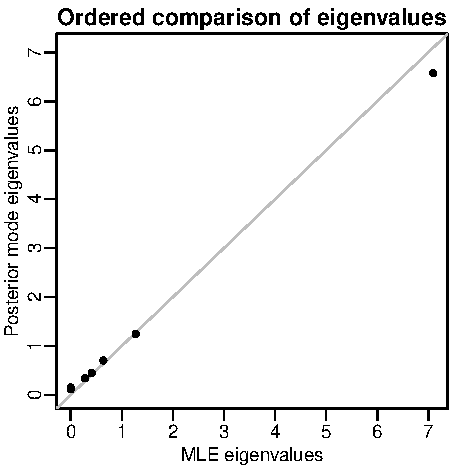
\includegraphics[width=2.5in]{eigenplot.pdf}}
\subfloat[]{\label{fig:spectral_comparison:contours}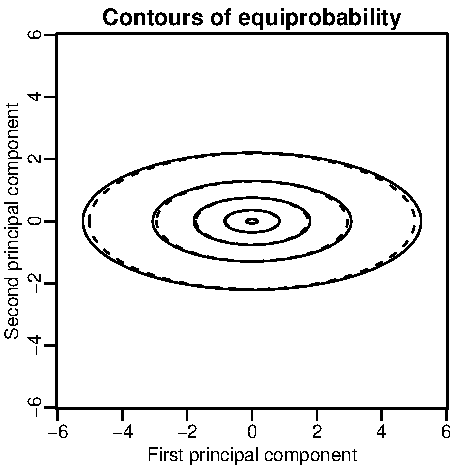
\includegraphics[width=2.5in]{contourplot.pdf}}
\end{center}
\caption{(a) Comparison of eigenvalues from the maximum likelihood fit and
  the posterior mode, using a spectral decomposition with
  $\Lambda_{[jj]} \sim \Gamma(2, 1)$. (b) Comparison of contours of equiprobability, viewing the first
  two components of the estimated posterior mode in the first two
  principal components from the maximum likelihood estimate. Lines
  correspond to 0.05, 0.25, 0.5, 0.75, and 0.95 probability of new
  observations have more extreme distances from the origin.
}
\label{fig:spectral_comparison}
\end{figure}

In order to assess in a technical sense the distance between the two
fits, Figure~\ref{fig:spectral_comparison:eigenvalues} visually shows the ordered eigenvalues. The eigenvalues demonstrate slight shrinkage
towards the prior mode, which in this case is 1. Under the null
hypothesis that the basic model is correct, the difference in
deviances is 2.90. (TODO: I'm not sure how many degrees of freedom to use
for this comparison, or really if it is even chi-squared).

Figure~\ref{fig:spectral_comparison:contours} shows a comparison of contours of
equiprobability. The posterior mode fit, when viewed in the first two
principal components of the maximum likelihood estimate, predicts a
similar pattern of variation to that of the MLE.

\begin{figure}
\begin{center}
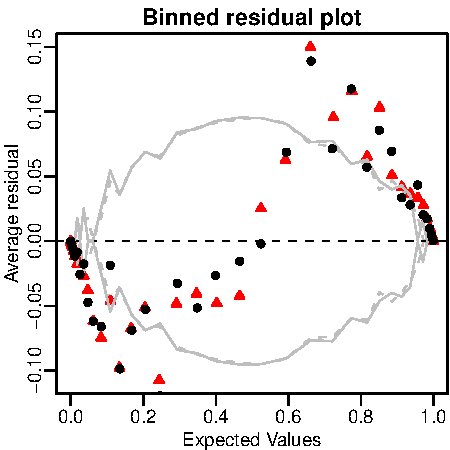
\includegraphics[width=3in]{binned_residuals.pdf}
\end{center}
\caption{Binned residual plots for maximum likelihood and posterior
  mode estimates. The black dots and solid gray lines correspond to
  the binned residuals and approximate 95\% confidence intervals for
  the MLE, while the red triangles and dashed lines are the same, respectively, for
  the posterior mode. \\
TODO: I think this plot should be redone, identifying which
observation ends up in which bin and making sure that they stay
consistent between the models. I suspect that the majority of the
difference in the plots arises from observations jumping bin boundaries.}
\label{fig:binned_residuals}
\end{figure}

However close the two fitted covariance matrices appear, more telling
are the associated predictions for each model. Taking the empirical
Bayes estimate of the modeled coefficients permits one to estimate the
expected value for each observation. From these, the Bayes estimator
of any actual dating decision is $y=1$ if the expected value is
greater than $0.5$, $0$ otherwise. Comparing these
predictions, the models agree for all but 25 out of 4427 data points,
or 99.4\% of the time. Figure~\ref{fig:binned_residuals} overlays binned
residual plots from both models, showing similar trends.

TODO: cross validation

\subsection{Full Bayesian inference}

TODO: section

\section{Availability}

\subsection{Installing the package}

\subsection{Obtaining the source code}

\subsection{License}

As \pkg{blmer} inherits code from \pkg{lme4}, it is available under
the GNU General Public License, versions 2.0 and greater. For a copy
of the license, visit \url{http://www.gnu.org/licenses/gpl.html}.

\bibliographystyle{plainnat}
\bibliography{blmer}

\end{document}
